%\begin{defin}
%A tree $(V,E)$ is called an \emph{binary tree} if $V$ contains one vertex $v$ of degree 2 and each other vertex in $V\setminus\lbrace v\rbrace$ has degree 3. The vertex $v$ of degree 2 is called the \emph{root} of the binary tree.
%\end{defin}

\begin{defin}
A \emph{binary rooted tree} $T^{(2)}$ is the graph $(V,E)$, where the vertex set 
\begin{equation*}
V:=\lbrace (b_i)_{i=1}^n\mid n\in \Z, n\geq 0, b_i\in\lbrace 0,1\rbrace\text{ for }1\leq i\leq n\rbrace,
\end{equation*}
is the set of all finite binary sequences including the empty sequence $(\emptyset)$. Two vertices $(b_i)_{i=1}^n,(c_i)_{i=1}^m\in V$ are adjacent if $|m-n|=1$ and the longer sequence can be obtained be concatenating 0 or 1 to the shorter sequence. Formally, the edge set $E$ of $T^{(2)}$ is defined as follows
\begin{equation*}
E:=\lbrace \lbrace(b_i)_{i=1}^n,(b'_i)_{i=1}^m\rbrace\in V\times V\mid m=n+1\text{ and } b_i=b'_i\text{ for } 1\leq i\leq n\rbrace.
\end{equation*}
For $n\in\N$, a vertex $(b_i)_{i=1}^n$ is \emph{on the $n$-th level} of $T^{(2)}$. The level of a vertex  is denoted by $|(b_i)_{i=1}^n|=n.$
\end{defin}
In the course of this thesis we will encounter many mappings with domain $\VT$. To increase readability, the image of a vertex $(\seq{b})\in\VT$ under a function $f\colon \VT\to X$ is denoted by $f(\seq{b})$ instead of $f((\seq{b}))$.
%The mapping $\beta\colon \VT\to\N$ defined by $\beta((\emptyset))=0$ and $\beta\left((b_i)_{i=1}^n\right)=\sum_{j=0}^{n-1} b_{n-j}2^j$ is a bijection. We define an total order on $\VT$ by
%\begin{equation*}
%(b_i)_{i=1}^n\leq(b'_i)_{i=1}^m :\Leftrightarrow \beta\left((b_i)_{i=1}^n\right)\leq\beta\left((b'_i)_{i=1}^m\right).
%\end{equation*}
%Note that $n<m$ suffices for $(b_i)_{i=1}^n<(b'_i)_{i=1}^m$.


\begin{thm}\label{thm:Binary Trees are Binary Trees}
The binary tree $\T$ fulfils the following two properties
\begin{thmlist}
\item $\T$ is connected and does not contain cycles. Hence $\T$ is a tree.
\item $\deg(\emptyset)=2$ and $\deg(v)=3$ for all vertices $v\in\VT\setminus\lbrace(\emptyset)\rbrace$.
\end{thmlist}
\end{thm}
\begin{proof}
The sequence $((\emptyset),(b_1),(b_1,b_2),\ldots,(\seq{b}))$ is a $(\emptyset)-(\seq{b})$-path for every vertex $(\seq{b})\neq(\emptyset)\in\VT.$ Hence, $\T$ is connected.\\
Assume $(u=v_0,\seq{v}=u)$ to be a cycle in $\T$, then there exists an index $i\in\lbrace 0,\ldots,n-1\rbrace$, such that $|v_i|=\max\lbrace |v_0|,|v_1|,\ldots,|v_{n-1}|\rbrace$. If $i=0$, the symbol $v_{i-1}=v_{-1}$ shall denote $v_{n-1}$, so that $v_i$ and $v_{i-1}$ are adjacent for $0\leq i\leq n-1$.\\
We find $|v_{i-1}|=|v_{i+1}|=|v_i|-1$ since the adjacency of $v_i$ to $v_{i\pm 1}$ implies $||v_i|-|v_{i\pm 1}||=1.$ If $v_i=(\seq[m]{b})$, there exists only one vertex on level $|v_i|-1$, which is adjacent to vertex $v_i$, namely $(\seq[m-1]{b})$. It follows, that
\begin{equation*}
v_{i-1}=(\seq[m-1]{b})=v_{i+1}.
\end{equation*}
Which contradicts the assumption, of $(u=v_0,\seq{v}=u)$ being a cycle and (i) is proven.\\
The second statement follows directly from the definition of $\T$.
\end{proof}

The diagram below visualizes the first four levels of $\T$. One identifies each vertex $v$ with the binary sequence obtained by concatenating the entries of the nodes one passes in the diagram when following the unique path from the root to $v$. The existence and uniqueness of this path is proven in \cref{thm:Unique Paths}. For example the black filled vertex corresponds to the sequence $(0,0,1,1)$. The path from the root to $(0,0,1,1)$ is highlighted in the diagram. 

\begin{center}
\mbox{
\beginpgfgraphicnamed{BinaryTree}
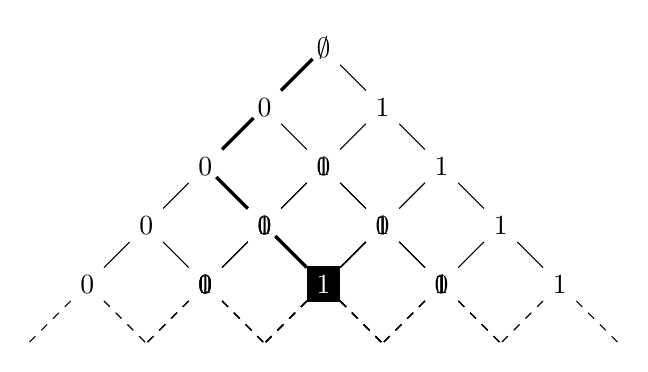
\begin{tikzpicture}[level distance=7.5mm]

\node (b) {$\emptyset$}
  child foreach \i in {0,1} {node {\i}
 {child foreach \j in {0,1} {node {\j}
 {child foreach \k in {0,1} {node {\k}
 {child foreach \l in {0,1} {node {\l}
 {child foreach \m in {0,1} {coordinate edge from parent[dashed]}}}}}}}}};

\node[very thick, fill=black, text=white] at (b-1-1-2-2) {1};	
\foreach \from/\to in {b/b-1,b-1/b-1-1,b-1-1/b-1-1-2,b-1-1-2/b-1-1-2-2}
	\node[very thick] at (\from) {}
	edge[very thick] (\to);
\end{tikzpicture}
\endpgfgraphicnamed
}
\end{center}

\begin{rem}
It is easy but rather technical to prove that the converse of \cref{thm:Binary Trees are Binary Trees} holds as well, i.e. for every tree $(V,E)$, such that $V$ contains a vertex $v_0$ of degree 2 and every other vertex $v\in V\setminus\lbrace v_0\rbrace$ is of degree 3, there exists a isomorphism $\varphi\colon V\to\VT.$ 
\end{rem}

\begin{defin}
For a given sequence $(\seq{b})$, the subgraph $(V,E)$ of $\T$ with the vertex set 
\begin{equation*}
V=\left\lbrace (\seq[n]{c},c_{n+1},\ldots,c_{n+k})\in\VT \,\middle\vert\, c_i=b_i \text{ for } 1\leq i\leq n\right\rbrace
\end{equation*}
containing all vertices corresponding to a sequence, that starts with $(\seq{b})$, and the edge set
\begin{equation*}
E=\mathcal{P}(V)\cap \VT
\end{equation*}
is denoted by $\ST{(\seq{b})}$.
\end{defin}

Note that adjacency is preserved in $\ST{(\seq{b})}$ for each vertex $v\in\ST{(\seq{b})}$ that is unequal to $(\seq{b})$, i.e. $\deg(v)=3$, whereas the degree of $(\seq{b})$ equals 2. As a consequence, $\ST{(\seq{b})}$ can be viewed as a binary tree.\\
In the diagram below the graph $\ST{(0)}$ is highlighted as a subtree of $\T$.

\begin{center}
\beginpgfgraphicnamed{Subtree}
\begin{tikzpicture}[level distance=7.5mm]
\node (b) {$\emptyset$}
  child foreach \i in {0,1} {node {\i}
 {child foreach \j in {0,1} {node {\j}
 {child foreach \k in {0,1} {node {\k}
 {child foreach \l in {0,1} {node {\l}
 {child foreach \m in {0,1} {coordinate edge from parent[dashed]}}}}}}}}};

\begin{scope}[bgn]
\node[draw=none] [above of=b]  {$\T$};
\node[draw=none] [above of=b-1] (ST0) {$\ST{(0)}$};
\end{scope}

\begin{pgfonlayer}{background}
\filldraw[st] (ST0.north) -- (b-1-1.north west) -- (b-1-1-1.west) -- (b-1-1-1-1.west) -- (b-1-1-1-1-1) -- (b-1-2-2-2-2) -- (b-1-2-2-2.east) -- (b-1-2-2.east) -- (b-1-2.north east) -- cycle; 
\end{pgfonlayer}
\end{tikzpicture}
\endpgfgraphicnamed
\end{center}

\begin{thm}\label{thm:Levels are preserved}
Every automorphism $\varphi\in\AutT$ preserves the levels of $\T$, i.e.
\begin{equation*}
\lvert \varphi(v)\rvert=\lvert v\rvert,\quad\forall v\in\VT.
\end{equation*}
\end{thm}

\begin{proof}
We prove the claim by induction on the level $n$ of a vertex $(\seq{b})\in\VT$. If $n$ equals 0, $(\seq{b})$ is the root of $\T$ and therefore the only vertex of degree 2. Hence, $\varphi(\seq{b})=(\seq{b})$ and the claim is proven.\\
We proceed by assuming the result to be shown for all vertices on levels less than $n$. Since, $\varphi(\seq{b})$ is adjacent to $\varphi(\seq[n-1]{b})$, the identity
\begin{equation*}
\big\lvert\lvert\varphi(\seq{b})\rvert-\lvert\varphi(\seq[n-1]{b})\rvert\big\rvert=1
\end{equation*}
holds. If $(\seq[n-1]{b})=(\emptyset),$ then $\varphi(\seq[n-1]{b})=(\emptyset)$. As a result, the image of $(\seq{b})$ under $\varphi$ is either $(0)$ or $(1)$, so that the statement is clear. If on the other hand $(\seq[n-2]{b})$ exists, then by the induction hypothesis this vertex is mapped  to the only vertex on level $n-2$, to which the vertex $\varphi(\seq[n-1]{b})$ is adjacent. Therefore, $(\seq{b})$ is mapped to a vertex on level $n$ and the claim is shown.
\end{proof}

Let
\begin{equation*}
\mathrm{L}(k):=\left\lbrace v\in\VT\middle\vert \lvert v\rvert=k\right\rbrace
\end{equation*}
be the set of all vertices on level $k\in\Z$, $k\geq 0$,  then \cref{thm:Levels are preserved} implies $\varphi(\mathrm{L}(k))=\mathrm{L}(k)$ for each automorphism $\varphi\in\AutT$. In the following we will study the action of $\AutT$ on $\mathrm{L}(k)$. For this purpose, let us consider the bijection $\beta_k\colon\mathrm{L}(k)\to\lbrace 1,2,\ldots 2^k\rbrace$ defined by 
\begin{equation*}
(\seq[k]{b})\mapsto 1+\sum_{i=1}^{k} b_i2^{k-i},
\end{equation*}
which identifies each vertex on level $k$ with an integer. Secondly, we consider the mapping $p_k:\AutT\to\mathfrak{S}_{2^k}$ which maps every $\varphi\in\AutT$ to the permutation $\sigma\in\mathfrak{S}_{2^k}$ defined by
\begin{equation*}
\sigma(i)=\beta_k(\varphi(\beta_k^{-1}(i))).
\end{equation*}
By construction the function $p_k$ maps each automorphism of $\T$ to its action on the vertices on level $k$. Assume $p_k(\varphi)=\sigma$ and $p_k(\psi)=\tau$, then
\begin{align*}
\beta_k((\varphi\circ\tau)(\beta_k^{-1}(i)))=&(\beta_k\circ\varphi\circ\tau\circ \beta_k^{-1})(i)=\\
=&((\beta_k\circ\varphi\circ \beta_k^{-1})\circ(\beta_k\circ\tau\circ \beta_k^{-1}))(i)=(\sigma\circ\tau)(i).
\end{align*}
Thus, $p_k$ is a homomorphism of groups.

\begin{defin}\label{def:Stabilizer Group}
The normal subgroup $\St{k}=\ker(p_k)$ of $\AutT$ is called \textit{$k$-th stabilizer group of $\T$}.
\end{defin}

\begin{pro}
Each automorphism $\varphi\in\St{k}$ preserves the first $k$ levels point-wise, i.e.
\begin{equation*}
\varphi\big\vert_{\bigcup_{i=0}^k\mathrm{L}(i)}=\id_{\bigcup_{i=0}^k\mathrm{L}(i)}.
\end{equation*}
\end{pro}
\begin{proof}
Assume there exists a vertex $(\seq{b})\in\bigcup_{i=0}^k\mathrm{L}(i)$, such that 
\begin{equation*}
\varphi(\seq{b})\neq (\seq{b})
\end{equation*}
and consider the vertex $(b_1,\ldots,b_n,b_{n+1},\ldots,b_k)$ on level $k$. The automorphism $\varphi$ will map this vertex to a vertex starting with $\varphi(\seq{b})$. Hence, 
\begin{equation*}
\varphi(\seq{b},b_{n+1},\ldots,b_k)\neq(b_1,\ldots,b_n,b_{n+1},\ldots,b_k),
\end{equation*}
which contradicts the premise $\varphi\in\St{k}$. 
\end{proof}